\documentclass[techrep, submit, noauthor,preface]{ipsj}
%\documentclass{ipsj}
 
\usepackage[dvipdfmx]{graphicx}
\usepackage{amsmath}
\usepackage{amsfonts}
\graphicspath{{./img/}}

\def\Underline{\setbox0\hbox\bgroup\let\\\endUnderline}
\def\endUnderline{\vphantom{y}\egroup\smash{\underline{\box0}}\\}
\def\|{\verb|}

\pagestyle{empty}
\begin{document}

\title{Parameter Unsharingを用いたMode Collapseの回避}

\paffiliate{EI}{慶應義塾大学 環境情報学部}
\paffiliate{GM}{慶應義塾大学 政策メディア研究科}

\author{勝又 海}{}{EI}
\author{小林 凌雅}{}{GM}

\maketitle
\thispagestyle{empty} 
%1
\begin{abstract}

  我々は発展著しいGANにおいて, その学習の安定化及びモデルの表現の多様化に寄与する学習手法を提案した.
  提案したParameter UnsharingでFeed Forward Networkによる回帰問題やGANによる混合正規分布の生成を実験し,
  学習の安定化に寄与することを検証した,
  また複数の学習手法の安定化手法と組み合わせた際に学習ごとに多様な表現を獲得することを確認した.

\end{abstract}

\section{序論}

自動運転の研究開発において, virtual evaluationの利用が活発になってきている.
virtual evaluationとは物理空間上で機械学習モデルの学習や評価を行うことが難しいタスクにおいて、
シミュレーション環境を用いて機械学習モデルの学習や評価を行う研究開発手法のことである.
近年のvirtual evaluationでは実運用での精度を担保するために
GANと呼ばれる手法を用いてシミュレーション環境をより現実的にしたり, 
データセットを拡充したりすることも多くなってきている.

GANとはGeneratorとDiscriminatorと呼ばれるニューラルネットワークを交互に学習させることでデータを生成する生成モデルである\cite{gan}. 他の生成モデルに比べて鮮明な画像が生成できることから画像生成のタスクにおいて頻繁に利用される
ようになってきている.
しかしながらGANの研究はまだまだ発展途上であり, いくつかの問題の存在が研究開発の発展を妨げている\cite{tutorial}.
1つはGANはGeneratorとDiscriminatorがお互いに競合しあい学習していく手法であり, 収束しないことがある.
また, Mode Collapseという現象により, 訓練に利用したデータとは似ても似つかない出力をするようになったり,
入力データを平均したような定数を出力するようになったりする.
本稿では、GANにおけるMode Collapseが引き起こされるという問題を回避する手法を提案する.

\section{関連研究}

{\bf Avoid Mode Collapse on GANs} Mode Collapseを回避する方法としてWGAN\cite{wgan}, Unrolled GAN\cite{unrolled}, PacGAN\cite{pacgan}などが提案されている.
WGANではWasserstein距離を定義し, Wasserstein距離に基いて学習を行っている.
Wasserstein距離は出力される画像の質と相関があるように定義されており, これを最小化するように学習することでMode Collapseを起こさず, 高品質の画像を出力できる.
Unrolled GANでは少し未来のDiscriminatorに対してGeneratorを学習させることで学習の安定化に成功した.
PacGANではミニバッチ中のデータ全てを
1つのデータとして捉えることでデータの分布を近似し, Mode Collapseの回避に成功した.

{\bf Regularization} ニューラルネットワークの文脈で使われることはそう多くはないが統計学の分野では
Parameter Sharing\cite{deeplearningbook}と呼ばれる手法が使われることがある.
これはモデルを学習させる際に別のモデルの重みに近づくように学習させる手法である.

{\bf Virtual Manipulation} 近年, ニューラルネットワークを用いた画像処理が行われるようになった.
例えば画風変換\cite{style}, 着色\cite{inpaint}などがある. またニューラルネットワークによって生成する画像を制御することも行われている\cite{pix2pixhd}.

\section{手法}

{\bf Mode Collapse} GANを学習していく中でGeneratorの出力が全て似たような画像になってしまう現象である.
多峰性の分布を学習するときや, Discriminatorだけが収束してしまったときなどに起こる.
これを回避するためにUnrolled GAN\cite{unrolled}, WGAN\cite{wgan}, PacGAN\cite{pacgan}などが用いられている.

{\bf Parameter Unsharing} 前項で上げられた手法には計算コストの大きさ, 一つの解に収束するため多様な表現の獲得ができない, Semi Supervised Learningでの利用ができないなど
の問題もある. 我々はこれらの課題を解決するためParameter Unsharingを提案した.
Parameter Unsharingは
学習の際に過去に学習したモデルの重みから遠ざかるように学習させることで別の最適解へ収束させる手法である.

GANのような複雑なモデルの解空間には多くの局所最適解が存在する.
分類や回帰であればlossに応じたaccuracyが得られるが, 
GANの場合には同じlossであったとしても全く異なる出力をすることが考えられる. 
この手法では別の局所最適解を探索させることでより良い出力をするモデルを得られる.


通常の目的関数にペナルティ項を加えて目的関数:
\begin{equation}
  \label{unshare}
  \tilde{\mathcal{L}}(\pmb{w}; \pmb{X}, \pmb{y}, \pmb{w}')
  =  - \frac{\alpha}{2} (\pmb{w} - \pmb{w}')^{\top}(\pmb{w} - \pmb{w}')  + \mathcal{L}(\pmb{w}; \pmb{X}, \pmb{y}),
\end{equation}
のパラメータの勾配は
\begin{equation}
  \label{nabla}
  \nabla_{w} \tilde{ \mathcal{L}}(\pmb{w}; \pmb{X}, \pmb{y}, \pmb{w}')
  =  - \alpha(\pmb{w} - \pmb{w}') + \nabla_{\pmb{w}}\mathcal{L}(\pmb{w}; \pmb{X}, \pmb{y})
\end{equation}
となる.
重みの更新式は
\begin{equation}
  \label{update}
  \pmb{w} \leftarrow \pmb{w} - \epsilon (- \alpha(\pmb{w} - \pmb{w}')
  + \nabla_{\pmb{w}}\mathcal{L}(\pmb{w}; \pmb{X}, \pmb{y}))
\end{equation}
となる.
式\ref{update}を簡単にすると
\begin{equation}
  \label{up}
  \pmb{w} \leftarrow (1 + \epsilon \alpha \pmb{w}) - \epsilon \alpha \pmb{w}'
  - \epsilon \nabla_{\pmb{w}}\mathcal{L}(\pmb{w}; \pmb{X}, \pmb{y}))
\end{equation}
となり, 式\ref{up}に従って最適化を行う.
過去のモデルから遠ざけると, もっとも距離が大きくなるのは重みの値が無限大のときである. 
重みが無限になった場合, lossは大きくなる. これを回避するために重み減衰の項を追加する.

{\bf Parameter Unsharing with MLP} 入力次元が1であるような回帰問題を想定する. 入力と出力はそれぞれ
$X = \{1, 2, 3, 4, 5,...\}$,$y = \{4, 16, 36, 64, 100,..\}$であり, これを満たす多項式は
$y = (2x)^{2}$もしくは$y = (-2x)^{2}$である. この二つのパラメータを推定させる.
\begin{equation}
  \label{regression}
  \mathcal{L}(\pmb{w}; \pmb{X}, \pmb{y}, \pmb{w}')
  =  - \frac{\alpha}{2} (\pmb{w} - \pmb{w}')^{\top}(\pmb{w} - \pmb{w}') + (f(\pmb{X}) - \pmb{y})^{\pmb{2}} 
\end{equation}      
と定義する.

{\bf Parameter Unsharing with GANs} 混合正規分布の学習を想定する. 目的関数は
\begin{equation}
  \label{gan}
  \begin{split}
    \mathcal{L}(\theta_{G}, \theta_{D}, \theta'_{G}) & =
    -\frac{\alpha}{2} (\theta_{G} - \theta'_{G})^{\top}(\theta_{G} - \theta'_{G}) \\
   & \quad +  \mathbb{E}_{x\sim p_{data}} [ \log(D(x; \theta_{D})) ]  \\
   & \quad + \mathbb{E}_{z\sim \mathcal{N}(0, I)} [ \log(1 - D(G(z;\theta_{G}); \theta_{D})) ]
   \end{split}
\end{equation}
と定義する.

\section{実験}

{\bf 多項式フィッテイング} 最適解が複数ある関数の当てはめを行った. 今回試したのは$y = ((2or-1)x)^2$である.パーセプトロンを確率的勾配法を用いて最適化を行った. Parameter Unsharingを使わずに最適化を行った場合には重みはランダムに-2もしくは2の値を取った. Parameter Unsharingを用いて最適化を行った場合は遠ざける対象のモデルの重みとは別の符号の値を取った.

{\bf GAN} 平均をずらした正規分布の混合分布から生成させたデータを生成させた. 生成させたの2,3,4つの正規分布の混合分布である.
いずれの場合もParameter Unsharingを繰り返し適用することで目標の分布を捉えることに成功している.

Mode Collapseの回避が可能であることを検証するとともに, 
学習がうまくいったと思われるモデルを利用してParameter Unsharingを行った場合の学習結果についても検証を行った. 
Unrolled Generative Adversarial Networkを用いて8つの正規分布の混合分布を学習させた. その後, 
学習させたモデルを用いてParameter Unsharingによる学習を行った. 学習したモデルの出力の散布図を図\ref{fig:unrolled}
に示す.

\begin{figure}[htb]
  \vspace{-0.5cm}
  \centering
    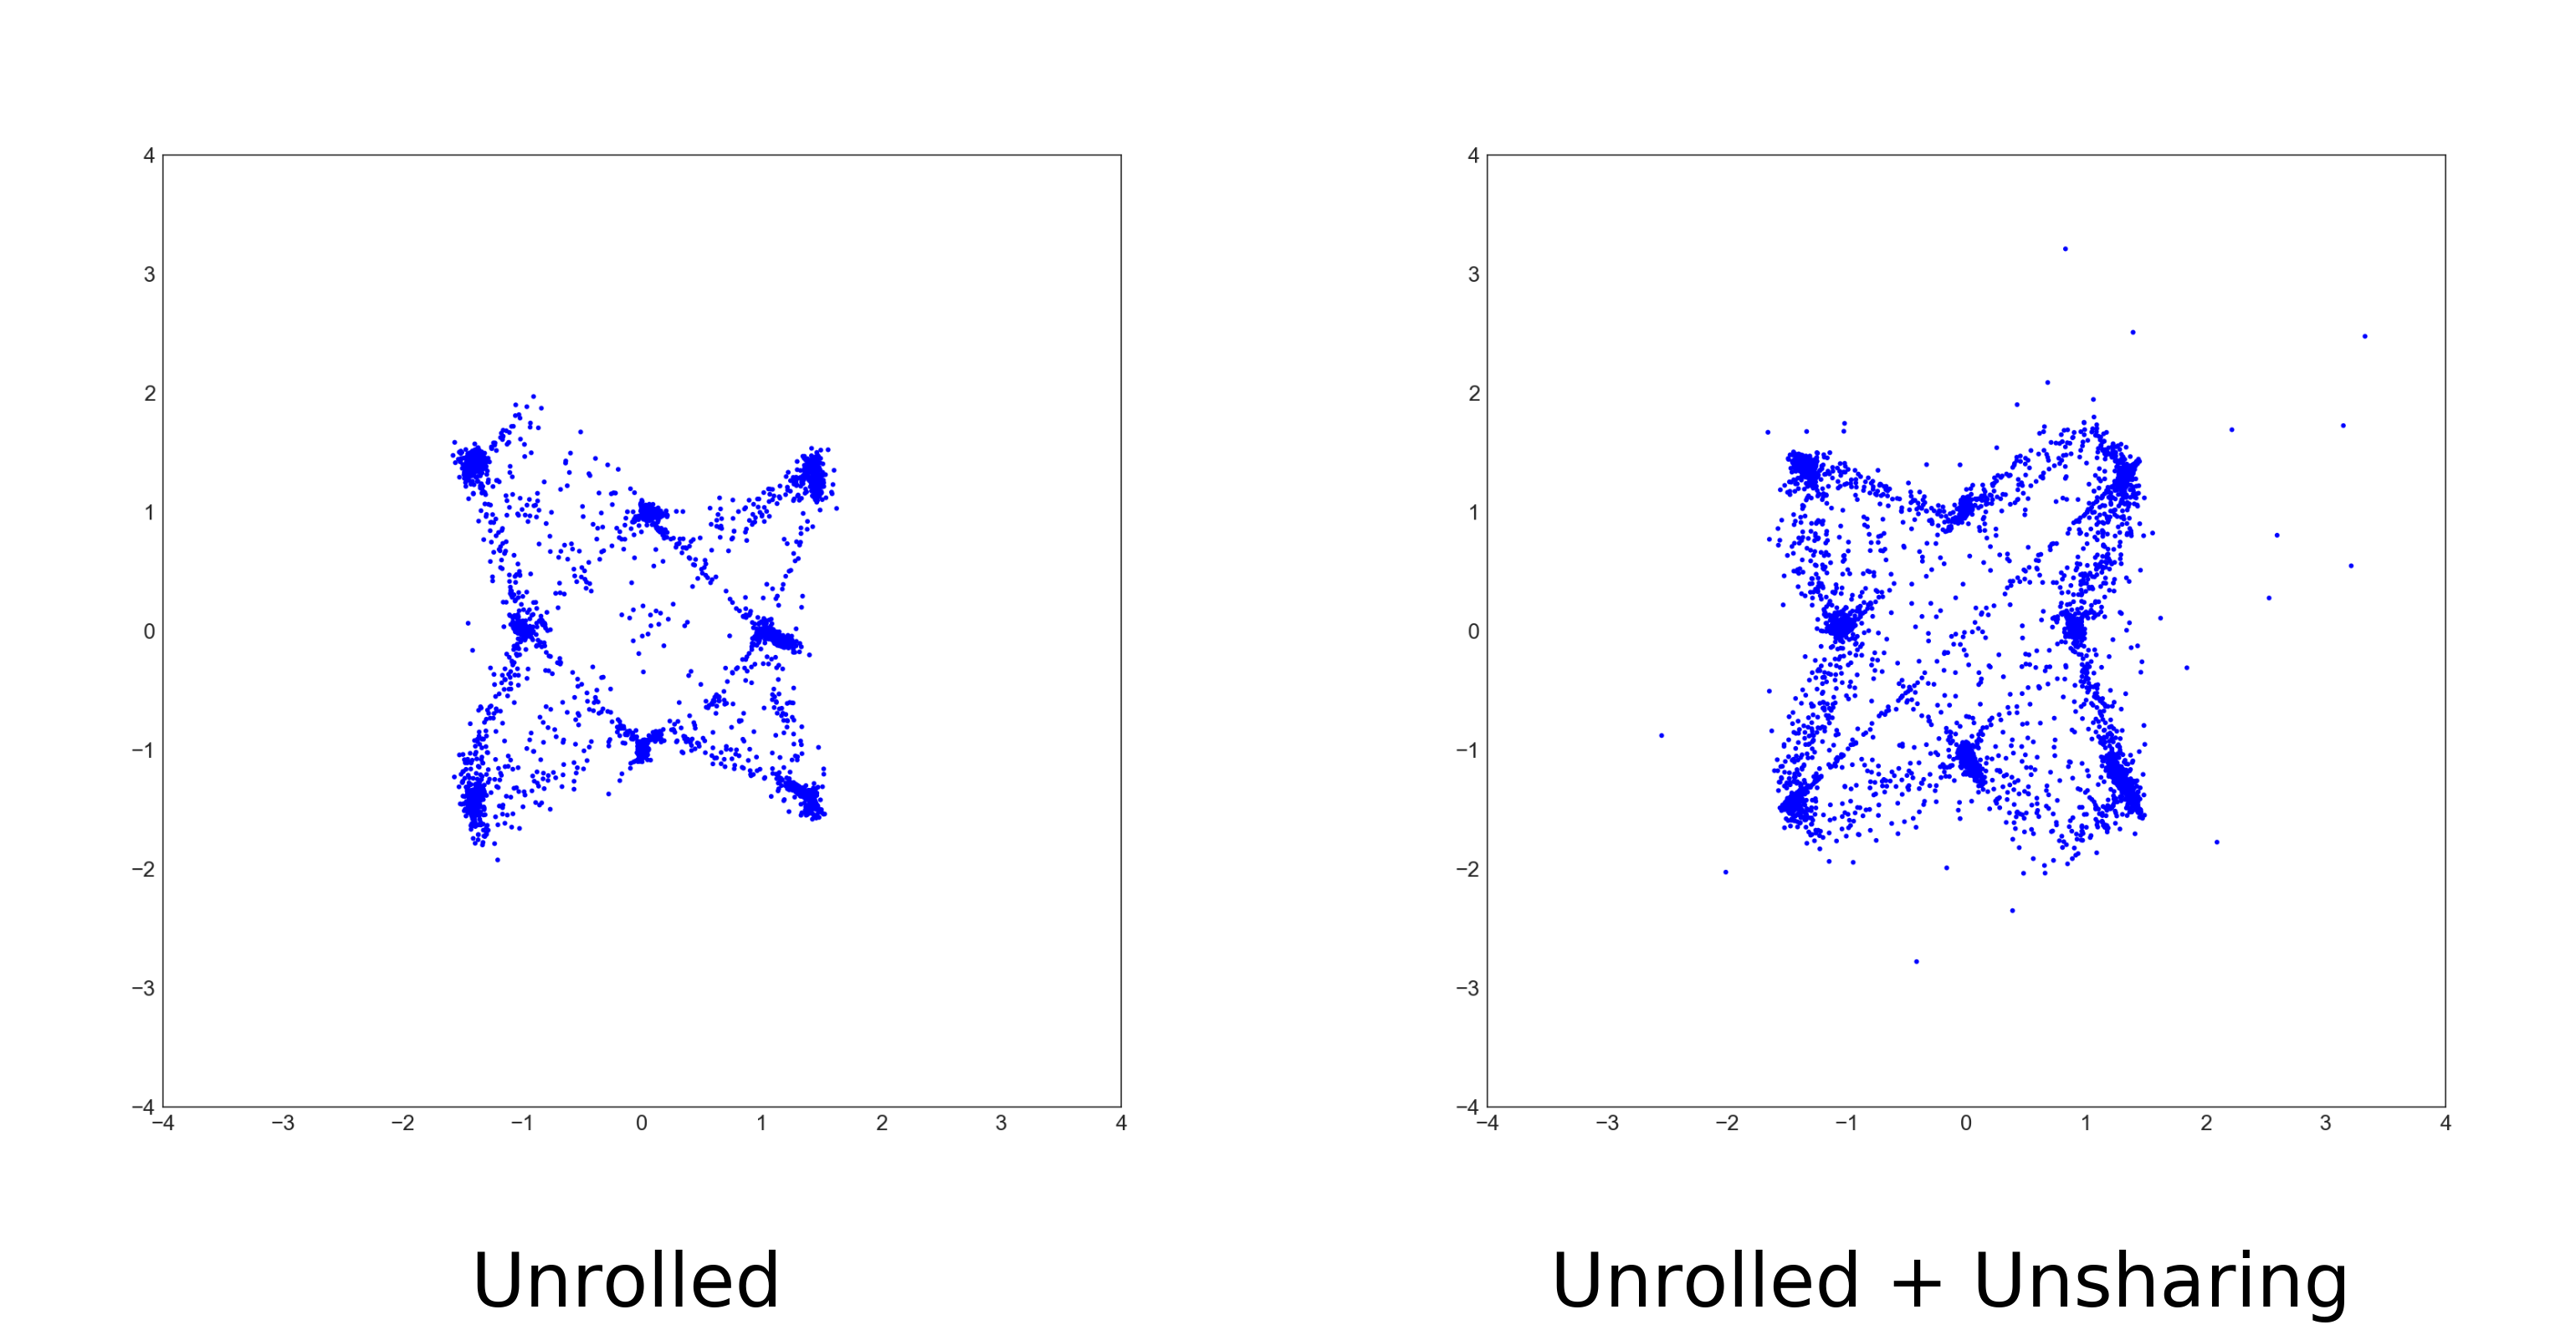
\includegraphics[height=3.5cm]{unrolled.png}
  \caption{学習したモデルの出力}
  \label{fig:unrolled}
  \vspace{-0.5cm}
\end{figure}

どちらも分布を捉えることができており, Parameter Unsharingを適用した場合には元のモデルとは少し異なる表現を獲得していることが分かる.

\section{今後の展望}

我々は提案した手法を用いて異なる最適解の探索が可能であることを検証した. 今回, いくつかのモデルに対して適用し, 検証を行ったが, 他のモデルに対する検証が不十分である. また, 学習の安定化に寄与する他の手法との比較が行えていない. 他の手法との比較を行う評価手法を研究し, 他の手法との比較を行う必要がある.

\bibliographystyle{ipsjunsrt}
\bibliography{ref}


\end{document}
